\documentclass[12pt,a4paper]{article}
\usepackage[utf8]{inputenc} %polskie znaki
\usepackage[T1]{fontenc}	%polskie znaki
\usepackage{amsmath}		%matematyczne znaczki :3
\usepackage{enumerate}		%Dodatkowe opcje do funkcji enumerate
\usepackage{geometry} 		%Ustawianie marginesow
\usepackage{graphicx}		%Grafika
\usepackage{wrapfig}		%Grafika obok textu
\usepackage{float}			%Allows H in figure
\usepackage{hyperref}		%Allows hyperlinks
%\pagestyle{empty} 			%usuwa nr strony
\usepackage{todonotes}		%Todo notatki
\usepackage{lipsum}         %Lorem text
\usepackage{ntheorem}   	% for theorem-like environments
\usepackage{mdframed}   	% for framing
\usepackage{subcaption}		% subfigure (image placing)
\usepackage{pdfcomment}		% Komentarze (z bazowego pdf'a)
\usepackage{xparse}			% New commands with optional arguments
\usepackage{ifthen}			% If then - funkcje!
\usepackage{expl3}			% Deklarowanie zmiennych
\usepackage{pgf}			% Aktualne rachunki \pgfmathparse{}
\usepackage{amsmath} 		% For mathematical symbols and structures
\usepackage{amsfonts}		% Zbiór liczb naturalnych + formatowanie
\usepackage{ulem}			% Przekreślony text
%\usepackage[colorlinks=true, linkcolor=blue, urlcolor=red, citecolor=green]{hyperref}
\usepackage{fontawesome5}
\usepackage{mathtools}

\newgeometry{tmargin=2cm, bmargin=2cm, lmargin=2cm, rmargin=2cm} 

%Counter commands{
	\newcounter{definicja}
	\setcounter{definicja}{1} 
	\newcounter{twierdzenie}
	\setcounter{twierdzenie}{1} 
	\newcounter{przyklady}
	\setcounter{przyklady}{1} 
	\newcounter{wnioski}
	\setcounter{wnioski}{1} 
	
	\newcommand{\counter}[1]{
		\arabic{#1} \stepcounter{#1} 
	}
	\newcommand{\counterreset}[1]{\setcounter{#1}{1}}
	%}

%Define styles{
	\theoremstyle{break}
	\theoreminframepreskip{0.5cm}
	\theoremheaderfont{\bfseries}
	\newmdtheoremenv[%
	linecolor=white,%
	innertopmargin=\topskip,
	shadowsize=0,%
	innertopmargin=5,%
	innerbottommargin=5,%
	leftmargin=10,%
	rightmargin=10,%
	backgroundcolor=gray!20,%
	innertopmargin=0pt,%
	ntheorem]{zad}{Zadanie}
	
	\mdfdefinestyle{zadanie}{
		linecolor=white,%
		innertopmargin=5,%
		innerbottommargin=5,%
		leftmargin=10,%
		rightmargin=10,%
		backgroundcolor=gray!20,%
		innertopmargin=8,
		innerbottommargin=8,
		skipabove = 5,
	}
	\mdfdefinestyle{wzor}{
		linecolor=cyan,%
		linewidth=2pt,%
		innertopmargin=8,
		innerbottommargin=8,
		leftmargin=10,%
		rightmargin=10,%
		backgroundcolor = white, 
		fontcolor = black,
		skipabove = 5,
		skipbelow = 5,
	}
	%}

%Zadania templatex%{
	\newcommand{\Obramowka}[1]{
		\begin{mdframed}[style=wzor]
			\centering #1
		\end{mdframed}
	}
	\newcommand{\Komentarz}[1]{
	\begin{mdframed}[style=zadanie]
		\textbf{Komentarz}\\
		#1
	\end{mdframed}
	}
	
	%}

% Set spacing before and after theorems
\setlength{\theorempreskipamount}{20pt}  % Space above the theorem
\setlength{\theorempostskipamount}{20pt} % Space below the theorem

\newtheorem{definition}{Definicja}[section]

\newtheorem{theorem}{Twierdzenie}[section]
\newtheorem{lemma}{Lemat}[section]
\newtheorem{wniosek}{Wniosek}[theorem]
\newtheorem{example}{Przykład}[section]
\newtheorem{exercise}{Ćwiczenie}[section]
\newtheorem{stwierdzenie}{Stwierdzenie}[section]
\newtheorem{obserwacja}{Obserwacja}[section]


\newcommand{\tg}{\text{tg}}
\newcommand{\ctg}{\text{ctg}}
\newcommand{\witw}{$\Leftrightarrow$}
\newcommand{\wynika}{$\Rightarrow$}
\newcommand{\UkladRownan}[2]{
	$\left\{
	\begin{array}{l}
		#1 \\
		#2
	\end{array}
	\right.$
}

\begin{document}
	% Strona tytułowa
	
	% Dodanie strony tytułowej
	\begin{titlepage}
		\centering
		\vspace{1cm}
		{\Huge\bfseries Matematyczne aspekty wyborów \par} 
		\vspace{1.5cm}
		{\large Na podstawie wykładu \par} 
		\vspace{0.5cm}
		{\Large Krzysztofa Ciesielskiego}\\
		\vspace{1cm}
		{\large Skrypt autorstwa}\\
		\vspace{0.5cm}
		{\Large Arkadiusza Dąbala}\\
		\vfill 
		{\large Wersja z dnia:}\\
		{\Large \today \par}  
		\vspace*{1cm}
	\end{titlepage}
	\newpage
	\tableofcontents
	\newpage
\section{Preliminaria}
\subsection{Jak wyglądają aktualnie wybory?}
\Komentarz{Materiał ten nie ma w żadnym stopniu charakteru politycznego, a wyłącznie charakter matematyczny.}

\begin{example}
Rozważmy poniższe dane, oparte na 6 partiach, 1000 głosach i 6 mandatów do rozdania:
\end{example}

\begin{tabular}{|c|c|c|c|c|c|c|}\hline
	Nazwa        & Głosy & $:1$ & $:2$ & $:3$ & $:4$ & Otrzymane mandaty\\\hline
	Filateliści  & 380   & \textbf{380} & \textbf{190} & \textbf{127} & 87   & 3\\\hline
	Gitarzyści   & 192   & \textbf{192} & \textbf{96}  & 64   &       & 2\\\hline
	Szachiści    & 180   & \textbf{180} & 90    &       &       & 1\\\hline
	Piłkarze     & 96    & \textbf{96}  & 48    &       &       & 1\\\hline
	Lotniarze    & 90    & 90    &       &       &       & 0\\\hline
	Kolejarze    & 62    & 62    &       &       &       & 0\\\hline
\end{tabular}\\

System ten działa w następujący sposób:

\begin{itemize}
	\item Liczby głosów dzielone są przez kolejne liczby naturalne dodatnie (tak jak w tabeli).
	\item Wybierane są z tej tabeli 6 największych liczb (wytłuszczony druk).
	\item Liczba mandatów zależy od liczby wytłuszczonych liczb w wierszu partii.
\end{itemize}

\begin{example}
	Rozważmy tę samą tabelę, ale załóżmy, że partia \textbf{Gitarzyści} nie przekroczyła progu $5\%$.
\end{example}

\begin{tabular}{|c|c|c|c|c|c|c|}\hline
	Nazwa        & Głosy & $:1$ & $:2$ & $:3$ & $:4$ & Otrzymane mandaty\\\hline
	Filateliści  & 380   & \textbf{380} & \textbf{190} & \textbf{127} & 87   & 3\\\hline
	\sout{Gitarzyści}  & \sout{192}  & \sout{192} & \sout{96}  & \sout{64}  & \sout{---} & \sout{---} \\\hline
	Szachiści    & 180   & \textbf{180} & \textbf{90}  &       &       & 2\\\hline
	Piłkarze     & 96    & \textbf{96}  & 48    &       &       & 1\\\hline
	Lotniarze    & 90    & \textbf{90}  &       &       &       & 1\\\hline
	Kolejarze    & 62    & 62    &       &       &       & 0\\\hline
\end{tabular}\\

\begin{example}
	Rozważmy następującą tabelę z 5 mandatami do rozdania:
\end{example}

\begin{tabular}{|c|c|c|c|c|c|}\hline
	Nazwa    & Głosy $:1$ & $:2$ & $:3$ & $:4$ & Mandaty\\\hline
	Rybacy   & \textbf{6000} & \textbf{3000} & \textbf{2000} & 1500 & 3\\\hline
	Myśliwi  & \textbf{5700} & \textbf{2850} & 1900  &       & 2\\\hline
	Artyści  & 1950          & 975           &       &       & 0\\\hline
\end{tabular}\\

Partia \textbf{Rybacy} prowadziła kampanię przeciwko \textbf{Myśliwym}, w wyniku czego liczba otrzymanych głosów zmieniła się następująco:
\begin{itemize}
	\item Partia \textbf{Rybacy} zyskała 400 głosów (+400)
	\item Partia \textbf{Myśliwi} straciła 600 głosów (-600)
	\item Partia \textbf{Artyści} zyskała 200 głosów (+200)
\end{itemize}

\begin{tabular}{|c|c|c|c|c|c|}\hline
	Nazwa    & Głosy $:1$ & $:2$ & $:3$ & $:4$ & Mandaty\\\hline
	Rybacy   & \textbf{6400} & \textbf{3200} & 2133 &       & 3\\\hline
	Myśliwi  & \textbf{5100} & \textbf{2550} & 1700 &       & 2\\\hline
	Artyści  & \textbf{2150} & 1075          &      &       & 0\\\hline
\end{tabular}\\

\Komentarz{Tym oto sposobem partia \textbf{Myśliwi} stracili jeden mandat na rzecz partii \textbf{Artyści}.}

\begin{example}
	Rozważmy wyniki głosowania dla dwóch partii z 6 mandatami do rozdania.
\end{example}

\begin{tabular}{|c|c|c|c|c|c|c|}\hline
	Nazwa        & Głosy $:1$ & $:2$ & $:3$ & $:4$ & $:5$ & Mandaty\\\hline
	Matematycy   & \textbf{1200} & \textbf{600} & \textbf{400} & \textbf{300} & \textbf{240} & 5\\\hline
	Politycy     & \textbf{201}  & 101         &       &       &       & 1\\\hline
\end{tabular}\\

Popatrzmy na głosy bezpośrednio na konkretnych kandydatów z każdej partii:

\begin{tabular}{|c|c|}\hline
	Nazwa   & Głosy\\\hline
	Kwadrat & \textbf{201}\\\hline
	Trójkąt & \textbf{200}\\\hline
	Stożek  & \textbf{200}\\\hline
	Walec   & \textbf{200}\\\hline
	Suma    & \textbf{200}\\\hline
	Iloczyn & 199\\\hline
\end{tabular} $\qquad\qquad\qquad\qquad\qquad$
\begin{tabular}{|c|c|}\hline
	Nazwa        & Głosy\\\hline
	Magister     & \textbf{35}\\\hline
	Magistra     & 34\\\hline
	Urzędnik     & 33\\\hline
	Urzędas      & 33\\\hline
	Pani Basia   & 33\\\hline
	Pan Andrzej  & 33\\\hline
\end{tabular}\\

\Komentarz{Tym oto sposobem mandatu nie otrzymuje \textbf{Iloczyn}, mimo że zdobył więcej głosów niż \textbf{Magister}.}

\begin{example}
	Rozważmy sytuację, w której państwo jest podzielone na dwa bloki, oba mające po $50\%$ wpływu na wyniki wyborów. Każdy blok ma przyznać po 4 mandaty.
\end{example}

\begin{center}
	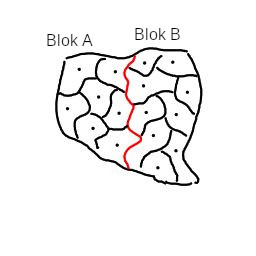
\includegraphics{5050.jpg}
\end{center}

W bloku A znajdowały się dwie partie: PZK (Partia Zwolenników Kawy) i PZH (Partia Zwolenników Herbaty), z których każda otrzymała po 25\% głosów w ogólnokrajowym głosowaniu. W bloku B znajdowała się partia PZA (Partia Zwolenników Alkoholu) oraz inne partie, które nie przekroczyły progu 5\%. Przedstawmy liczbę uzyskanych głosów w PZA:

\begin{tabular}{|c|c|}\hline
	Nazwa       & Głosy\\\hline
	Żubr        & \textbf{19995}\\\hline
	Żubrówka    & \textbf{2}\\\hline
	Soplica     & \textbf{2}\\\hline
	Pan Tadeusz & \textbf{1}\\\hline
\end{tabular}\\

\Komentarz{I tym oto sposobem wygrywają osoby, które dostają 2 lub 1 głos.}

\subsection{\href{http://www.racjonalista.pl/kk.php/s,9848/k,3}{Prawo Ciesielskiego}}

Rozważmy głosowanie względem 2 partii z 7 mandatami:

\begin{tabular}{|c|c|c|c|c|c|c|}\hline
	Nazwa        & Głosy:1 & :3 & :5  & :7  & :9  & Mandaty\\\hline
	Kelnerzy     & \textbf{1050} & \textbf{350} & \textbf{210} & 150 & 117  & 4\\\hline
	Sportowcy    & \textbf{1008} & \textbf{336} & 202  & 144 &      & 3\\\hline
\end{tabular}\\

Partia \textbf{Sportowcy} postanowiła się rozdzielić na dwie partie i startować osobno:

\begin{tabular}{|c|c|c|c|c|c|c|}\hline
	Nazwa        & Głosy:1 & :3 & :5  & :7  & :9  & Mandaty\\\hline
	Kelnerzy     & \textbf{1050} & \textbf{350} & \textbf{210} & 150 & 117  & 3\\\hline
	Piłkarze     & \textbf{504}  & \textbf{168} & 101  &     &      & 2\\\hline
	Siatkarze    & \textbf{504}  & \textbf{168} & 101  &     &      & 2\\\hline
\end{tabular}\\

\Komentarz{Tym oto sposobem partia \textbf{Sportowcy} zdobyła większość.}

	
\newpage

\section{Treść właściwa}
\subsection{Metody głosowania (system wyborczy)}

Wprowadźmy kilka oznaczeń, niech: \\
\\ $W$ - zbiór wszystkich wyborców, \\
$K$ - zbiór wszystkich kandydatów.
\begin{itemize}
	\item Ten sam układ głosów (zestaw głosów) daje ten sam wynik (funkcja).
	\item Każdy układ głosów daje jakiś wynik (może być $\emptyset$).
\end{itemize}

\begin{definition}[Model]
	Model to układ głosów (z przyporządkowanymi wyborcami).
\end{definition}

\begin{definition}[Metoda anonimowa]
	Metoda jest anonimowa, \textit{wtedy i tylko wtedy} (w skrócie: \witw), gdy wszyscy wyborcy są traktowani tak samo, \witw $\forall_{x,y \in W}$ zamiana głosów $x$ i $y$ nie zmienia wyniku.
\end{definition}

\Komentarz{Alternatywnie, metoda nie jest anonimowa \witw $\exists_{x,y \in W}$ takie, że zamiana głosów $x$ i $y$ \textit{istotnie} zmienia wynik.}

\begin{definition}[Metoda neutralna]
	Metoda jest neutralna, \witw wszyscy kandydaci są traktowani tak samo, \witw $\forall_{x,y \in K}$ zamiana ról $x$ i $y$ nie zmienia wyniku.
\end{definition}

\Komentarz{Alternatywnie, metoda nie jest neutralna \witw $\exists_{x,y \in K}$ takie, że zamiana ról $x$ i $y$ \textit{istotnie} zmienia wynik, dokładniej definiując:\\
jeśli $\exists{k_1,k_2\in K}: W_1=\{w_{1},w_{2},\dots,w_{i}\}$ głosowali na $k_1$, a $W_2=\{w_{i+1},w_{i+2},\dots,w_{j}\}$ głosowali na $k_2$ to jeżeli kandydaci Ci "zamienią się" wyborcami (zbiorami $W_1,W_2$), to $k_1$ i $k_2$ zamienią się wynikami.}

\begin{definition}
	Trzy rodzaje metod ze względu na wyniki:
\end{definition}

\begin{enumerate}[1)]
	\item Metoda zwycięzcy (MZ) – wybiera zwycięzcę (zwycięzców),
	\item Metoda porządkowa (MP) – wynik to słaby porządek na zbiorze $K$,
	\item Metoda rozdziału (MR) – wynik to podział pewnych dóbr między kandydatów.
\end{enumerate}
\subsubsection{Metoda zwyciężcy}
\begin{definition}[Klasyczna metoda zwycięzcy]
	Klasyczna metoda zwycięzcy (klasyczna MZ) polega na tym, że każdy wyborca głosuje na dokładnie jednego kandydata. Zbiór
	$$\Sigma = \{m:W\rightarrow K\}$$
	jest zbiorem modeli, gdzie $m$ jest modelem. Klasyczną metodę zwycięzcy możemy opisać funkcją
	$$f: \Sigma \rightarrow P(K).$$
\end{definition}

\begin{definition}[Semi-klasyczna metoda zwycięzcy]
	Semi-klasyczna MZ polega na tym, że każdy wyborca głosuje na co najmniej jednego kandydata:
	$$\Sigma = \{m:W\rightarrow P(K)\setminus \emptyset\}.$$
	Metodę tę można opisać funkcją
	$$f: \Sigma \rightarrow P(K).$$
\end{definition}

\begin{definition}[Metoda efektywna]
	Metoda zwycięzcy jest efektywna \witw zawsze wyłania przynajmniej jednego zwycięzcę.
\end{definition}

\begin{example}[Przykłady metod głosowania]
	\textbf{Metody klasyczne:}
\end{example}
\begin{enumerate}[1)]
	\item Dyktatura – $\exists_{\;p \in W}$: wynik jest tożsamy z głosem $p$.
	\item Monarchia – dany kandydat $k \in K$ wygrywa niezależnie od głosowania.
	\item Metoda większości – wygrywa kandydat (lub kandydaci), który(a) otrzymał(a) najwięcej głosów.
	\item Metoda bezwzględnej większości – wygrywa kandydat $k \in K$, który otrzymał co najmniej $\lfloor\frac{\# W}{2}\rfloor + 1$ głosów.
	\item Metoda super większości – wygrywa kandydat, który uzyskał co najmniej $q$ głosów, gdzie $q > \frac{\# W}{2}$.
	\item Metoda status quo – \textit{Założenie:} $\exists$ pewien stan z jednym zwycięzcą.
	\\ Głosowanie metodą większości (lub super większości):
	\begin{itemize}
		\item jeśli metoda daje wynik, zwycięża "nowy" kandydat,
		\item jeśli metoda nie daje wyniku, zwycięża dotychczasowy kandydat.
	\end{itemize}
	Przykład: referendum.
	\item Metoda większości ważonej – $(W = \{a_1,\dots,a_n\})$, gdzie głos $a_i$ ma wagę $w_i \geq 0$. Wygrywa ten, kto otrzyma ponad $\frac{w_1 + \dots + w_n}{2}$ punktów.
	\item Metoda głosowania blokowego – $W = W_1 \cup \dots \cup W_n$, gdzie $W_k$ to zbiór wyborców bloku. $W_k$ podejmuje decyzję większością głosów. W przypadku remisu wybierają zwycięzcę w $W_k$. Głos z $W_k$ ma wagę $i_k$. Wygrywa kandydat z największą liczbą punktów.
	
	\textbf{Metody semi-klasyczne:}
	\item Metoda n-głosów – każdy wyborca głosuje na $n$ kandydatów, a zwycięża ten, kto uzyska najwięcej głosów.
	\item Szeroka metoda n-głosów - każdy głosuje na n kandydatów, ale mamy n zwyciężców (lub więcej w przypadku remisu na ostatnim "wygrywającym" miejscu)
	
	\textbf{Metoda ani klasyczna, ani semi-klasyczna:}
	\item Metoda punktowa – każdy wyborca $w \in W$ ma do rozdysponowania $p$ punktów $(p \in \mathbb{N})$ między kandydatów. Zwycięża kandydat z największą liczbą punktów.
\end{enumerate}

\begin{definition}[Metoda decyzyjna]
	Metoda zwycięzcy jest decyzyjna \witw w każdym modelu wyłania dokładnie jednego zwycięzcę.
\end{definition}

\begin{definition}[Metoda prawie decyzyjna]
	Metoda zwycięzcy jest prawie decyzyjna \witw w każdym modelu wyłania co najwyżej jednego zwycięzcę. Sytuacja, w której nie ma zwycięzcy, zachodzi wtedy, gdy więcej niż jeden kandydat uzyskał tę samą, najwyższą liczbę punktów.
\end{definition}

\begin{exercise}[Z ćwiczeń]
	Zbadaj kto jest zwycięzcą w głosowaniu przez 99 osób na kandydatów: \textbf{Anastazy}, \textbf{Bermudy}, \textbf{Cezary}, jeśli otrzymano następujące wyniki metodą porządkową:
\end{exercise}

	\begin{tabular}{|c|c|}\hline
		Liczba głosów	& Wynik porządkowy\\\hline
		18        		& ABC\\\hline
		15    			& ACB\\\hline
		24     			& BAC\\\hline
		8 				& BCA\\\hline
		16     			& CAB\\\hline
		18 				& CBA\\\hline
	\end{tabular}\\
	
\begin{exercise}
	Dane są wyniki głosowania:\\\\
	\begin{tabular}{|c|c|}\hline
		Imię		& Liczba głosów\\\hline
		Jaś        	& 100\\\hline
		Małgosia    & 1\\\hline
	\end{tabular}\\\\
	Zrób tak, by Małgosia wygrała.
\end{exercise}

\begin{exercise}
	Uzupełnij tabelę:\\
	\begin{tabular}{|c|c|c|c|}\hline
		& Anonimowa & Neutralna & Efektywna\\\hline
		Dyktatura   &-&+&+\\\hline
		Monarchia   &+&-&+\\\hline
		Metoda Większości &+&+&+\\\hline
	\end{tabular}\\
\end{exercise}




	\begin{definition}[Kryterium jednoznacznej bezwzględnej większości]
		Metoda zwycięzcy (MZ) spełnia kryterium jednoznacznej bezwzględnej większości, \textit{wtedy i tylko wtedy}, gdy kandydat, który otrzyma ponad 50\% głosów, jest jedynym zwycięzcą.
	\end{definition}
	
	\begin{stwierdzenie}
		Mamy klasyczną metodę zwycięzcy, taką że $\# K=2$, a głosowanie odbywa się według zasady bezwzględnej większości. Wówczas metoda jest prawie decyzyjna.
	\end{stwierdzenie}
	
	\textit{Dowód:}
	\begin{enumerate}[1$^\circ$]
		\item Załóżmy, że liczba wyborców $\# W$ jest nieparzysta - OK.
		\item Liczba wyborców $\# W$ jest parzysta:
		\begin{itemize}
			\item jeden kandydat ma więcej niż 50\% głosów - OK.
			\item remis, czyli obaj mają po 50\% - nie ma zwycięzcy (dlatego metoda jest prawie decyzyjna).
		\end{itemize}
		\begin{flushright}$\square$\end{flushright}
	\end{enumerate} 
	
	\begin{stwierdzenie}
		Metoda jest decyzyjna $\Rightarrow$ metoda jest prawie decyzyjna.
	\end{stwierdzenie}
	
	\begin{definition}[Metoda monotoniczna ze względu na zwycięzcę]
		\textbf{Z:} MZ - klasyczna lub semi-klasyczna.
		Metoda jest monotoniczna ze względu na zwycięzcę, \textit{wtedy i tylko wtedy}, gdy kandydat $A$ jest zwycięzcą, a jeśli wybierzemy kandydata $B$ różnego od $A$ ($B\neq A$) oraz jego grupę wyborców, to jeśli ta grupa zmieni swoje głosy bez straty dla $A$ (czyli zmiana nastąpi zgodnie z następującymi dozwolonymi operacjami):
		
		\begin{tabular}{|c|c|c|}
			\hline
			M & $\Rightarrow$ & N \\\hline
			A B & $\Rightarrow$ & A B \\\hline
			- - & $\Rightarrow$ & - - \\\hline
			+ + & $\Rightarrow$ & + + \\\hline
			- + & $\Rightarrow$ & + - \\\hline
		\end{tabular}
		
		to: $\Rightarrow$ $A$ nadal wygrywa.
	\end{definition}
	
	\Komentarz{Czyli, jeżeli ktoś, kto nie głosował na zwycięzcę ($A$), a głosował na kandydata $B$, zmieni swój głos na zwycięzcę ($A$), to ($A$) nadal wygrywa.}
	
	\begin{definition}[Metoda kwoty]
		MZ klasyczna lub semi-klasyczna jest metodą kwoty (większości kwalifikowanej), \textit{wtedy i tylko wtedy}, gdy istnieje $q$ (kwota), taka że liczba głosów o tej własności, że kandydat $A$ jest zwycięzcą \textit{wtedy i tylko wtedy}, gdy $A$ otrzymał co najmniej $q$ głosów.
		
		\Komentarz{Często kwota wyrażana jest w procentach, a wówczas stosuje się nieraz nierówność słabą.}
	\end{definition}
	\begin{theorem}[Maya - \textit{Kenneth Maya, 1952r}]
		\textbf{Z:} Klasyczna metoda zwycięzcy oraz $\# K = 2$. Jeżeli metoda ta jest metodą:
		\begin{enumerate}[(1)]
			\item anonimową
			\item neutralną
			\item monotoniczną ze względu na zwycięzcę
			\item prawie decyzyjną
		\end{enumerate}
		$\Rightarrow$ jest metodą bezwzględnej większości.
	\end{theorem}
	
	\textit{Dowód:}
	Załóżmy, że $A,B$ to kandydaci.\\
	$\overset{(1)}{\Rightarrow}$ interesują nas liczby głosów, które otrzymali kandydaci. Załóżmy:\\
	$A$ - $a$ głosów\\
	$B$ - $b$ głosów\\
	Rozpatrzmy zatem przypadki:\\
	\begin{enumerate}[1$^\circ$]
		\item $\# W = 2n$ (parzysta), rozważmy dwa podprzypadki:
		\begin{enumerate}[a)]
			\item Jeśli $a=n$, $b=n$.\\
			\textbf{Hipoteza:} $A$ wygrywa (analogicznie, jeżeli nie wygrywa $B$), a metoda jest neutralna, to przy wymianie wyborców $\overset{(2)}{\Rightarrow}$ $B$ wygrywa (nie wygrywa $A$) $\Rightarrow$ $A$ i $B$ wygrywają jednocześnie (nie wygrywa żaden) $\Rightarrow$ co prowadzi do \faBolt (bo żaden z nich nie ma ponad 50\%).
			
			\item Jeśli $a>b$.\\
			\textbf{Hipoteza:} $B$ wygrywa, wtedy $a-b$ wyborców zmienia głosy z $A$ na $B$, $\overset{(3)}{\Rightarrow}$ $B$ dalej wygrywa. Teraz $B$ ma $a$ głosów, $\overset{(2)}{\Rightarrow}$ $A$ wygrywa, $\overset{(4)}{\Rightarrow}$ $A$ wygrywa i ma ponad połowę głosów.
		\end{enumerate}
		
		\item Niech $\# W = 2n+1$ (nieparzysta).\\
		Niech $a>b$.\\
		\textbf{Hipoteza:} $B$ wygrywa, $a-b$ wyborców zmienia głosy i, jak w 1a), udowadniamy, że $B$ musi mieć ponad połowę głosów.
	\end{enumerate}
	
	Tak więc zawsze wygrywa ten, kto ma ponad połowę głosów.
	\begin{flushright}$\square$\end{flushright}
	\subsubsection{MZU - Metoda zakładająca uporządkowanie}
	\begin{definition}[Metoda zakładająca uporządkowanie]
		Metoda zwycięzcy jest metodą zakładającą uporządkowanie (MZU) \textit{wtedy i tylko wtedy}, gdy $\forall_{w\in W}$ ustala $K$ kandydatów w liniowym porządku, a jego głos zależy od tego porządku.
	\end{definition}
	
	\textbf{Zapis:}\\\\
	$A\overset{w,m}{<}B$ w modelu $m$ oznacza, że wyborca $w$ stawia $B$ wyżej niż $A$.\\
	$A\overset{w}{<}B$ - gdy wiadomo, jaki model.
	
	\begin{example}
		\begin{enumerate}[1.]
			\item Metoda punktów Bordy (Jean Charles de Borda, 1733–1799, inżynier wojskowy) – Każdy wyborca przydziela punkty od $n-1$ do 0:
			1. $n-1$
			2. $n-2$
			$\vdots$
			$n-1$ - 1
			$n$ - 0\\
			Zwycięża ten, kto otrzyma największą liczbę punktów.
			
			\item Metoda Hare'a (Sir Thomas Hare, 1806–1891, Anglia, prawnik, 1857 r.) – Polega na odrzucaniu tego kandydata (tych kandydatów), który ma najmniej pierwszych miejsc, i głosowaniu dalej (listy pozostają z usunięciem odrzuconego kandydata), aż ktoś uzyska ponad $50\%$ głosów. Gdy następuje remis i nie ma kogo odrzucić, wszyscy wygrywają.
			
			\item Metoda Coombsa (Clyde Coombs, 1912–1988, USA, psycholog) – Wypisujemy kolejność, odrzucamy kandydata, który ma najwięcej ostatnich miejsc, i głosujemy dalej, aż ktoś uzyska ponad $50\%$ pierwszych miejsc. Gdy nie można nikogo odrzucić, wygrywają wszyscy, którzy pozostali.
			
			\item Metoda odrzuceń ostatniego – Jak w metodzie Coombsa, przy czym odrzucamy „do oporu”. Gdy nie można nikogo więcej odrzucić, wygrywają wszyscy, którzy pozostali.
			
			\begin{example}
				Różnica między metodą Coombsa a metodą odrzucania ostatniego.\\
				
				\textbf{Metoda Coombsa}\\
				\begin{tabular}{|c|c|c|c|}\hline
					Liczba: & 4 & 2 & 3 \\\hline
					I pozycja & C & \textbf{B} & \textbf{B} \\\hline
					II pozycja & A & C & A \\\hline
					III pozycja & B & A & C \\\hline
				\end{tabular}\\\\
				Wygrywa $B$, bo ma ponad 50\% pierwszych miejsc.\\\\
				
				\textbf{Metoda odrzuceń ostatniego}\\
				\begin{tabular}{|c|c|c|c|}\hline
					Liczba: & 4 & 2 & 3 \\\hline
					I pozycja & C & B & B \\\hline
					II pozycja & \xout{A} & C & A \\\hline
					III pozycja & \sout{B} & \xout{A} & C \\\hline
				\end{tabular}\\\\
				Kolejność odrzuceń: B, A, C – C wygrywa.
			\end{example}
			
			\item Metoda Copelanda (Arthur H. Copeland, 1898–1970, matematyk) – Porównujemy parami kandydatów. Ten, kto więcej razy zostaje oceniony wyżej, dostaje 1 pkt, a w przypadku remisu obaj dostają po 0,5 pkt.
			
			$\#\{m:A\overset{m}{<}B\}$\\
			$\#\{m:B\overset{m}{<}A\}$\\
			
			Decyduje suma punktów (zwycięzców może być więcej niż jeden).
			
			\item Metoda turniejowa (Z: $\# W = 2n+1$ nieparzysta) – $k_1$ porównujemy z $k_2$ (metodą powyżej), następnie porównujemy z $k_3$ itd.
			
			\item Metoda pozycyjna – $P(p_1, p_2, \dots, p_n)$, gdzie $p_1\geq p_2 \geq \dots \geq p_n$. 
			1 – $p_1$ punktów,
			2 – $p_2$ punktów itd.\\
			Zwycięża ten z największą liczbą punktów.\\
			
		\end{enumerate}
			
			
		\textbf{UWAGA – w szczególności:}\\
		Metoda Bordy: $P(n-1, n-2, \dots, 1, 0)$\\
		Metoda większości: $P(1,0, \dots, 0)$\\
		Metoda $k$ głosów: $P(\underset{\text{k razy}}{1,1,\dots,1}, 0, \dots, 0)$
	\end{example}
		
		\begin{definition}[Monotoniczność ze względu na transpozycję]
			MZU jest monotoniczna ze względu na transpozycje \witw $\forall_{M-\text{model}} \forall_{w\in W} \forall_{A,B\in K}$, jeśli w $M$ głosuje się $[\Delta, B, A, *]$ i w $M$ wygrywa $A$, to w $N$, gdzie zmiana polega na $[\Delta, A, B, *]$, również wygrywa $A$.
		\end{definition}
		
		\Komentarz{Zmiana polega na zamienieniu kolejności uporządkowania $A$ i $B$. Dodatkowo porządek ten był na wykładzie zapisany pionowo. $\begin{bmatrix}
				\Delta\\
				A\\
				B\\
				*
			\end{bmatrix}$
		}
		
		{\textbf{Umowa:}} Jeśli nie jest zaznaczone inaczej, to w $K,W$ różne oznaczenia oznaczają różnych kandydatów (wyborców).
		
		\begin{definition}[Słaba zasada Pareto]
			MZU spełnia słabą zasadę Pareto \witw $\forall_M (\exists_{A,B\in K}\forall_{w\in W} A\overset{w,M}{<}B) \Rightarrow A$ nie wygrywa w $M$.
		\end{definition}
		
		\begin{definition}[Kandydat Condorceta]
			$A\in K$ jest kandydatem Condorceta (zwycięzcą Condorceta) \witw w "bezpośrednich porównaniach" $A$ jest lepszy od każdego innego kandydata \witw $\forall_{B \in K}: B\neq A \#\{w: B\overset{w,M}{<}A\}>\#\{w: B\overset{w,M}{>}A\}$.
		\end{definition}
		
		\begin{definition}[Przegrany Condorceta]
			$A\in K$ to przegrany Condorceta (w modelu $M$) \witw $\forall_{B \in K}: B\neq A \#\{w: B\overset{w,M}{<}A\}<\#\{w: B\overset{w,M}{>}A\}$.
		\end{definition}
		
		\begin{definition}[Kryterium Condorceta]
			Metoda spełnia kryterium Condorceta \witw $\forall_M:$ Istnieje kandydat Condorceta (w $M$) $\Rightarrow A$ - jedyny zwycięzca w $M$.
		\end{definition}
		
		\begin{definition}[Kryterium przegranych Condorceta]			
			Metoda spełnia kryterium przegranych Condorceta \witw $\forall_M:$ Istnieje przegrany Condorceta $A$ w $M$ $\Rightarrow A$ nie wygrywa w $M$.
		\end{definition}
		
		\begin{definition}[Metoda jednoznacznie większościowa]
			Metoda jest jednoznacznie większościowa \witw $\forall_M$ kandydat $A$ w $M$ ma ponad połowę pierwszych miejsc $\Rightarrow A$ - jedyny zwycięzca.
		\end{definition}
		
		\begin{definition}[Metoda słabo niezależna od ubocznych opcji]
			Metoda słabo niezależna od ubocznych opcji spełnia warunek niezależności porażki od ubocznych opcji (spełnia słaby warunek $IIA$) \witw
			
			$\forall_{A,B\in K} \forall_{M,N - modele}$ spełnia 
			$\begin{bmatrix}
				\forall_{w\in W} (B\overset{w,M}{<}A) \text{\witw} (B\overset{w,N}{<}A) \\
				\text{A wygrywa w M, B nie wygrywa w M}		 
			\end{bmatrix}$	$\Rightarrow$ B nie wygrywa w N.\\\\
			
			Innymi słowy: zmiany nie wpływające na relacje przegrany-zwycięzca nie mogą dać przegrywającemu zwycięstwa.		
			
		\end{definition}
		
		\begin{theorem}
			MZU, anonimowa, neutralna $\Rightarrow$ metoda nie jest decyzyjna.
		\end{theorem}
		\textit{Dowód.} Rozważmy $\# K = 2$, $\# W = 2n$ i otrzymane głosy.\\
		
		\begin{tabular}{|c|c|c|}\hline
			Głosy&n&n\\\hline
			1&A&B\\\hline
			2&B&A\\\hline
		\end{tabular}\\\\
		\textbf{Hipoteza:} Metoda decyzyjna to np. wygrywa $A \Rightarrow$ wygrywa $B$ \faBolt\\
		Analogicznie zachodzi dla $A$.
		
		\begin{flushright}$\square$\end{flushright}
		
		\begin{example}[Paradoks Condorceta]
			Rozważmy następującą tabelę:\\
			\begin{tabular}{|c|c|c|c|}\hline
				Głosy&9&10&11\\\hline
				1&A&B&C\\\hline
				2&B&C&A\\\hline
				3&C&A&B\\\hline
			\end{tabular}\\
			
			Zachodzi $A>B$, $B>C$, $C>A$. Mamy więc grę w "kamień, papier, nożyce."
		\end{example}
		
		\begin{theorem}
			MZU spełnia kryterium Condorceta $\Rightarrow$ jest jednoznacznie większościowa.
		\end{theorem}
		\textit{Dowód.} A ma ponad połowę pierwszych miejsc $\Rightarrow$ A - kandydat Condorceta $\Rightarrow$ A jest jedynym zwycięzcą.		
		
		\begin{flushright}$\square$\end{flushright}
		
		\begin{theorem}
			MZU spełnia słabe $IIA$, a $A$ spełnia kryterium Condorceta $\Rightarrow$ spełnia słabą zasadę Pareto.
		\end{theorem}
		\textit{Dowód.} Rozważmy $M$ $\forall_{W} A\overset{w,M}{<}B \overset{?}{\Rightarrow}$ $A$ nie wygrywa w $M$.
		
		Rozważmy model $N$: dla każdego wyborcy przesuwamy $A$ i $B$ na szczyt, $[B,A,reszta]$ $A\overset{w,M}{<}B$ \witw $A\overset{w,N}{<}B$.
		
		W $N$: $B$ jest kandydatem Condorceta.
		
		W $N$: $B$ jest jedynym zwycięzcą, $B$ wygrywa, $A$ nie wygrywa. 
		
		$\overset{\textbf{Słabe IIA}}{\Rightarrow}$ $A$ nie wygrywa w $M$.
		\begin{flushright}$\square$\end{flushright}
		
		\begin{theorem}
			MZU, monotoniczna ze względu na transpozycje, \witw $\forall_{M - \text{model}} \forall_{A\in K} \forall_{B_1,\dots,B_n\in A} (A\neq B, \text{ ale może być } B_i=B_j)$
			$\forall_{w_1,\dots,w_n\in W}$ (może być $w_i=w_j$)
			
			Jeżeli w modelu $M$ wygrywa $A$, to model $N$ utworzony przez $[\Delta, B_i, A, *] \rightarrow [\Delta, A, B_i, *]$ dla $i=1,\dots,n$ $\Rightarrow$ w $N$ dalej wygrywa $A$.
			
		\end{theorem}
		
		\textit{Dowód.} $\Leftarrow$ oczywiste.
		
		$\Rightarrow$ Stosujemy założenie $n$ razy (robimy $n$ skoków i dalej wygrywa $A$).
		
		\begin{example}
			
		\end{example}
		
		\begin{enumerate}[1.]
			\item Metoda Blacka (1908-1991, ekonomista) - jeśli istnieje kandydat Condorceta, to on wygrywa. Jeśli nie istnieje, stosujemy punkty Bordy.
			\item Metoda Condorceta - jeśli istnieje kandydat, który w "bezpośrednim porównaniu" wygrywa lub remisuje z każdym innym, \witw on jest zwycięzcą.
			\item Metoda nominacji - każdy, kto ma co najmniej jedno pierwsze miejsce, wygrywa.
			\item Metoda ostatnich miejsc - każdy, kto nie ma żadnego ostatniego miejsca, wygrywa.
			\item Metoda prezydencka - rozważamy dwóch kandydatów z największą liczbą pierwszych miejsc. Porównujemy ich "bezpośrednio". Jeśli na drugim miejscu jest remis, wszyscy z drugiego miejsca "przechodzą do finału" i tam stosujemy metodę Copelanda.
		\end{enumerate}
		
		Metoda punktów Bordy jest monotoniczna ze względu na transpozycję.
		
		$A$ wygrywa. Niech $A$ dostanie 1 punkt więcej. Innym się nie zwiększyło $\Rightarrow$ $A$ dalej wygrywa.
		
	\newpage
	\section{Deser}
	W sumie to deseru jeszcze nie ma, ale ma być na ostatnim wykładzie!!! 
		
	\begin{center}
		 {\fontsize{30}{36}\selectfont\faBirthdayCake}
	\end{center}
	

	
	
\end{document}